% =============================================================================
% SECTION 5 - DYNAMIQUE DU MOUVEMENT CIRCULAIRE
% Bloc 7 (2 heures - Semaine 8)
% =============================================================================

\section{Dynamique du mouvement circulaire}
\label{sec:circulaire}

% =============================================================================
\subsection{Retour sur l'accélération centripète}
\label{subsec:rappel-centripete}
% =============================================================================

Au chapitre précédent, nous avons découvert un résultat surprenant : un objet qui se déplace en cercle à vitesse \textit{constante} possède quand même une accélération! Cette accélération, appelée \textbf{centripète}, est dirigée vers le centre du cercle.

\begin{definition}[title=Rappel : accélération centripète]
Un objet en mouvement circulaire uniforme (vitesse constante en module) possède une accélération dirigée vers le centre :

\begin{equationimportante}
\begin{equation}
    a_c = \frac{v^2}{r} = \omega^2 r
    \label{eq:accel-centripete}
\end{equation}
\end{equationimportante}

où :
\begin{itemize}
    \item $v$ est la vitesse (tangentielle) de l'objet
    \item $r$ est le rayon de la trajectoire circulaire
    \item $\omega$ est la vitesse angulaire (en rad/s)
\end{itemize}
\end{definition}

\begin{remarque}[title=Pourquoi une accélération si la vitesse est constante?]
Souvenez-vous : l'accélération mesure le \textbf{changement de vitesse}, et la vitesse est un \textbf{vecteur}. Un vecteur peut changer de deux façons :
\begin{itemize}
    \item En \textbf{module} (la « grandeur » change) $\rightarrow$ accélération tangentielle
    \item En \textbf{direction} (l'orientation change) $\rightarrow$ accélération centripète
\end{itemize}

Dans un mouvement circulaire uniforme, seule la direction change. La vitesse « tourne » constamment, ce qui constitue un changement, donc une accélération.
\end{remarque}

% =============================================================================
\subsection{La force centripète : cause de l'accélération}
\label{subsec:force-centripete}
% =============================================================================

Maintenant, appliquons la deuxième loi de Newton. S'il y a une accélération vers le centre, alors il \textit{doit} y avoir une force résultante vers le centre!

\begin{definition}[title=Force centripète]
La \textbf{force centripète} est la force résultante nécessaire pour maintenir un objet sur une trajectoire circulaire :

\begin{equationimportante}
\begin{equation}
    \boxed{F_c = ma_c = m\frac{v^2}{r} = m\omega^2 r}
    \label{eq:force-centripete-def}
\end{equation}
\end{equationimportante}

Cette force est \textbf{toujours dirigée vers le centre} de la trajectoire circulaire.
\end{definition}

\begin{attention}[title=Point crucial : la force centripète n'est PAS une nouvelle force!]
C'est l'erreur la plus fréquente dans ce chapitre. La force centripète n'est \textbf{pas} un nouveau type de force à ajouter sur votre DCL!

C'est simplement le \textbf{nom} qu'on donne à la composante de la force résultante qui pointe vers le centre du cercle. Cette force peut être fournie par :

\begin{center}
\renewcommand{\arraystretch}{1.4}
\begin{tabular}{|l|l|}
\hline
\rowcolor{bleuclair} \textbf{Situation} & \textbf{Force qui fournit $F_c$} \\
\hline
Balle au bout d'une ficelle & Tension de la ficelle \\
\hline
Voiture dans un virage plat & Frottement des pneus \\
\hline
Satellite en orbite & Gravité \\
\hline
Passager dans un manège & Normale du siège \\
\hline
Eau dans un seau qu'on fait tourner & Normale du fond du seau \\
\hline
Lune autour de la Terre & Attraction gravitationnelle \\
\hline
\end{tabular}
\end{center}

\textbf{Sur un DCL, on dessine la vraie force (tension, frottement, normale...), jamais « $F_c$ » comme force séparée!}
\end{attention}

\begin{center}
\begin{tikzpicture}[scale=1.1]
    % Titre
    \node[font=\bfseries] at (0, 3.8) {Trois situations, même principe};
    
    % Situation 1 : Balle sur ficelle
    \begin{scope}[xshift=-4.5cm]
        % Trajectoire
        \draw[dashed, gray] (0, 0) circle (1.5);
        \fill (0, 0) circle (2pt);
        
        % Ficelle et balle (position à 45°)
        \draw[thick, brown] (0, 0) -- (1.06, 1.06);
        \shade[ball color=blue!50] (1.06, 1.06) circle (0.15);
        
        % Tension (vers le centre)
        \draw[-{Stealth[length=3mm]}, very thick, orange] (1.06, 1.06) -- (0.35, 0.35);
        \node[orange, below right] at (0.5, 0.5) {$\vec{T}$};
        
        % Vitesse (tangente, perpendiculaire à la ficelle)
        \draw[-{Stealth[length=2.5mm]}, thick, purple] (1.06, 1.06) -- (0.36, 1.76);
        \node[purple, left] at (0.3, 1.7) {$\vec{v}$};
        
        \node[below, text width=2.5cm, align=center] at (0, -2) {\small Balle sur ficelle \\ $F_c = T$};
    \end{scope}
    
    % Situation 2 : Voiture dans virage
    \begin{scope}[xshift=0cm]
        % Trajectoire circulaire (même style que les autres)
        \draw[dashed, gray] (0, 0) circle (1.5);
        
        % Centre du virage
        \fill (0, 0) circle (2pt);
        \node[below] at (0, -0.2) {\scriptsize centre};
        
        % Voiture (rectangle plus grand, à 135°)
        \begin{scope}[shift={(-1.06, 1.06)}, rotate=-45]
            \draw[thick, fill=blue!30, rounded corners=2pt] (-0.3, -0.15) rectangle (0.3, 0.15);
            % Roues
            \fill[gray!70] (-0.25, -0.18) rectangle (-0.15, -0.12);
            \fill[gray!70] (0.15, -0.18) rectangle (0.25, -0.12);
            \fill[gray!70] (-0.25, 0.12) rectangle (-0.15, 0.18);
            \fill[gray!70] (0.15, 0.12) rectangle (0.25, 0.18);
        \end{scope}
        
        % Frottement (vers le centre)
        \draw[-{Stealth[length=3mm]}, very thick, green!60!black] (-1.06, 1.06) -- (-0.35, 0.35);
        \node[green!60!black, right] at (-0.3, 0.7) {$\vec{f}$};
        
        % Vitesse (tangente)
        \draw[-{Stealth[length=2.5mm]}, thick, purple] (-1.06, 1.06) -- (-1.76, 0.36);
        \node[purple, below left] at (-1.6, 0.5) {$\vec{v}$};
        
        \node[below, text width=2.5cm, align=center] at (0, -2) {\small Voiture en virage \\ $F_c = f$};
    \end{scope}
    
    % Situation 3 : Satellite
    \begin{scope}[xshift=4.5cm]
        % Terre
        \shade[ball color=blue!40] (0, 0) circle (0.5);
        \node[font=\tiny, white] at (0, 0) {Terre};
        
        % Orbite
        \draw[dashed, gray] (0, 0) circle (1.5);
        
        % Satellite (plus grand et reconnaissable)
        \draw[thick, fill=gray!50] (-0.1, 1.35) rectangle (0.4, 1.65); % corps
        \draw[thick, fill=blue!30] (-0.45, 1.42) rectangle (-0.1, 1.58); % panneau gauche
        \draw[thick, fill=blue!30] (0.4, 1.42) rectangle (0.75, 1.58); % panneau droit
        
        % Gravité (vers le centre)
        \draw[-{Stealth[length=3mm]}, very thick, red] (0.15, 1.5) -- (0.15, 0.7);
        \node[red, left] at (0.1, 1.0) {$\vec{F}_g$};
        
        % Vitesse
        \draw[-{Stealth[length=2.5mm]}, thick, purple] (0.15, 1.5) -- (0.95, 1.5);
        \node[purple, above] at (0.6, 1.55) {$\vec{v}$};
        
        \node[below, text width=2.5cm, align=center] at (0, -2) {\small Satellite en orbite \\ $F_c = F_g$};
    \end{scope}
\end{tikzpicture}
\end{center}

% =============================================================================
\subsection{La « force centrifuge » : un mirage}
\label{subsec:force-centrifuge}
% =============================================================================

Vous avez certainement ressenti cette sensation d'être « poussé vers l'extérieur » dans un virage serré ou sur un manège. Cette sensation est si forte qu'on lui a donné un nom : la « force centrifuge ». Mais existe-t-elle vraiment?

\begin{attention}[title=La force centrifuge n'existe pas!]
Dans un référentiel inertiel (comme le sol), \textbf{aucune force} ne vous pousse vers l'extérieur d'un virage.

Ce que vous ressentez, c'est votre \textbf{inertie} : votre corps tend à continuer en ligne droite (première loi de Newton), tandis que la voiture tourne sous vous. C'est le siège et la ceinture qui vous \textit{tirent} vers l'intérieur pour vous faire tourner avec la voiture.

\textbf{Résumé :} La « force centrifuge » est une \textbf{sensation}, pas une force réelle. Elle n'apparaît que si vous analysez le mouvement depuis un référentiel \textit{non inertiel} (comme l'intérieur de la voiture qui tourne), ce que nous ne faisons pas dans ce cours.
\end{attention}

\begin{remarque}[title=Analogie pour comprendre]
Imaginez que vous êtes debout dans un autobus qui freine brusquement. Vous avez l'impression d'être « poussé vers l'avant ». Mais personne ne vous pousse! C'est simplement que votre corps continue tout droit (inertie) pendant que l'autobus ralentit sous vos pieds.

C'est exactement la même chose dans un virage : vous continuez « tout droit » pendant que la voiture tourne.
\end{remarque}

% =============================================================================
\subsection{Méthode de résolution}
\label{subsec:methode-circulaire}
% =============================================================================

Pour résoudre des problèmes de mouvement circulaire, on applique le même algorithme qu'avant, avec une particularité : on choisit un axe pointant \textbf{vers le centre} du cercle.

\begin{definition}[title=Algorithme pour le mouvement circulaire]

\textbf{Étape 1 --- DCL}
\begin{itemize}
    \item Identifier toutes les forces \textbf{réelles} (poids, normale, tension, frottement...)
    \item Ne \textbf{jamais} ajouter « $F_c$ » comme force séparée!
\end{itemize}

\textbf{Étape 2 --- Axes}
\begin{itemize}
    \item Un axe vers le \textbf{centre} du cercle (direction de $\vec{a}_c$)
    \item Un axe perpendiculaire (souvent vertical ou tangentiel)
\end{itemize}

\textbf{Étape 3 --- Équations de Newton}
\begin{itemize}
    \item Selon l'axe vers le centre : $\displaystyle\sum F_{\to centre} = ma_c = m\frac{v^2}{r}$
    \item Selon l'autre axe : $\sum F_\perp = 0$ (ou $ma_\perp$ s'il y a accélération)
\end{itemize}

\textbf{Étape 4 --- Résolution algébrique}
\end{definition}

\begin{exemple}{Voiture dans un virage}{voiture-virage}
Une voiture de masse $m = \SI{1200}{kg}$ prend un virage horizontal de rayon $r = \SI{50}{m}$. Le coefficient de frottement statique entre les pneus et la route est $\mu_s = 0{,}8$.

Quelle est la vitesse maximale à laquelle la voiture peut négocier ce virage sans déraper?

\tcblower

\textbf{\underline{Analyse physique}}

Pour que la voiture tourne, il faut une force centripète dirigée vers le centre du virage. Sur une route horizontale, cette force est fournie par le \textbf{frottement statique} entre les pneus et la route.

Si la voiture va trop vite, le frottement nécessaire dépasse le frottement maximal disponible $\rightarrow$ la voiture dérape vers l'extérieur.

\textbf{\underline{DCL (vue de derrière la voiture)}}

\begin{center}
\begin{tikzpicture}[scale=1.3]
    % Route
    \fill[gray!30] (-2.5, 0) rectangle (2.5, -0.2);
    \draw[thick] (-2.5, 0) -- (2.5, 0);
    
    % Voiture (vue de derrière, simplifiée)
    \draw[thick, fill=blue!20, rounded corners=2pt] (-0.8, 0.05) rectangle (0.8, 0.85);
    \draw[thick, fill=gray!50] (-0.75, -0.05) rectangle (-0.45, 0.1); % roue gauche
    \draw[thick, fill=gray!50] (0.45, -0.05) rectangle (0.75, 0.1); % roue droite
    
    % Centre de masse
    \fill[blue!50] (0, 0.45) circle (3pt);
    
    % Forces
    % Poids (vers le bas)
    \draw[-{Stealth[length=3mm]}, very thick, red] (0, 0.45) -- (0, -0.9);
    \node[red, left] at (-0.1, -0.3) {$\vec{F}_g$};
    
    % Normale (vers le haut)
    \draw[-{Stealth[length=3mm]}, very thick, green!60!black] (0, 0.45) -- (0, 1.8);
    \node[green!60!black, left] at (-0.1, 1.2) {$\vec{N}$};
    
    % Frottement (vers le centre = vers la gauche sur ce schéma)
    \draw[-{Stealth[length=3mm]}, very thick, orange] (0, 0.45) -- (-1.8, 0.45);
    \node[orange, above] at (-1.0, 0.55) {$\vec{f}_s$};
    
    % Indication du centre
    \draw[dashed, gray] (-2.8, 0.45) -- (-2.1, 0.45);
    \node[left, font=\small] at (-2.8, 0.45) {Centre du virage};
    
    % Axes (déplacés à droite, bien séparés)
    \draw[-{Stealth}, thick] (2.0, 0.45) -- (2.0, 1.5) node[right] {$y$};
    \draw[-{Stealth}, thick] (2.0, 0.45) -- (1.0, 0.45) node[below right] {$x$};
    \node[font=\scriptsize, below] at (1.5, 0.3) {(vers centre)};
\end{tikzpicture}
\end{center}

\textbf{\underline{Équations}}

Selon $y$ (vertical) : $\sum F_y = 0$
\[
    N - mg = 0 \quad \Rightarrow \quad N = mg
\]

Selon $x$ (vers le centre) : $\sum F_x = ma_c$
\[
    f_s = m\frac{v^2}{r}
\]

\textbf{\underline{Condition de non-dérapage}}

Pour que la voiture ne dérape pas, il faut $f_s \leq f_{s,max} = \mu_s N = \mu_s mg$.

À la vitesse maximale, $f_s = f_{s,max}$ :
\[
    \mu_s mg = m\frac{v_{max}^2}{r}
\]

Les masses s'annulent (la vitesse maximale ne dépend pas de la masse!) :
\[
    v_{max} = \sqrt{\mu_s g r}
\]

\textbf{\underline{Application numérique}}
\[
    v_{max} = \sqrt{0{,}8 \times 9{,}81 \times 50} = \sqrt{392{,}4} = \SI{19{,}8}{m/s} \approx \boxed{\SI{71}{km/h}}
\]

\textbf{Remarques importantes :}
\begin{itemize}
    \item La vitesse maximale ne dépend \textbf{pas} de la masse du véhicule.
    \item Sur route mouillée ($\mu_s \approx 0{,}5$) : $v_{max} \approx \SI{56}{km/h}$.
    \item Sur glace ($\mu_s \approx 0{,}1$) : $v_{max} \approx \SI{25}{km/h}$!
\end{itemize}
\end{exemple}

% -----------------------------------------------------------------------------
\subsubsection{Application maritime : cargaison dans un virage}
% -----------------------------------------------------------------------------

Lorsqu'un navire effectue un virage, une force centripète doit être exercée pour le maintenir sur sa trajectoire circulaire. D'où vient cette force?

\begin{remarque}[title=Origine de la force centripète sur un navire]
Contrairement à une voiture qui utilise le frottement des pneus, un navire vire en \textbf{deux étapes} :

\begin{enumerate}
    \item Le \textbf{safran} (gouvernail), braqué à l'arrière, crée un \textbf{couple de lacet} qui fait pivoter le navire.
    \item Ce pivotement donne à la coque un \textbf{angle de dérive} par rapport à l'écoulement. La coque agit alors comme un profil hydrodynamique et génère une \textbf{force latérale vers l'intérieur du virage} : c'est la force centripète.
\end{enumerate}

\begin{center}
\begin{tikzpicture}[scale=1.0]
    % Navire pivoté (proue vers tribord = droite, angle de dérive ~ 12°)
    \begin{scope}[rotate=-12]
        \draw[thick, fill=gray!20] (-0.5, -2) -- (0.5, -2) -- (0.6, 0) 
            -- (0.3, 1.5) -- (0, 1.8) -- (-0.3, 1.5) -- (-0.6, 0) -- cycle;
        \node at (0, -0.5) {\small Navire};
        
        % Safran (braqué vers tribord)
        \draw[very thick, blue!70] (0, -2) -- (0.6, -2.6);
        \node[blue!70, below right] at (0.5, -2.5) {\small Safran};
        
        % Force sur le safran (vers bâbord = gauche = extérieur du virage)
        \draw[-{Stealth}, thick, orange] (0.3, -2.3) -- (-1.5, -2.3);
        \node[orange, above] at (-0.8, -2.2) {\small $\vec{F}_{\text{safran}}$};
    \end{scope}
    
    % Direction de la trajectoire (verticale = direction du mouvement du CdM)
    \draw[-{Stealth}, very thick, purple] (0, 2.0) -- (0, 3.8);
    \node[purple, left] at (-0.15, 3.0) {$\vec{v}$ (trajectoire)};
    
    % Ligne de l'axe du navire (prolongée au-delà de la proue, pour montrer β)
    \draw[thin, gray, dashed] (0, 2.0) -- ({2.5*sin(12)}, {2.0+2.5*cos(12)});
    
    % Angle de dérive β (entre trajectoire verticale et axe du navire)
    \draw[thick, <->] (0, 3.5) arc (90:78:1.5);
    \node[font=\small, right] at (0.35, 3.5) {$\beta$};
    
    % Force centripète (force latérale de la coque, vers le centre = vers la droite)
    \draw[-{Stealth}, very thick, red] (0, 0) -- (3.0, 0);
    \node[red, above] at (2.2, 0.15) {$\vec{F}_c$ (coque)};
    
    % Centre du virage
    \fill (5.5, 0) circle (3pt);
    \node[below] at (5.5, -0.2) {\small Centre du virage};
    
    % Trajectoire courbée
    \draw[dashed, gray] (0, 2.0) arc (90:40:5.5);
\end{tikzpicture}
\end{center}

Le safran ne fournit donc \textbf{pas} la force centripète : il initie la rotation. C'est la \textbf{coque en dérive}, présentant un angle d'attaque $\beta$ à l'écoulement, qui génère par pression hydrodynamique la force centripète nécessaire au mouvement circulaire.
\end{remarque}

\begin{exemple}{Cargaison sur le pont d'un navire virant}{navire-virage}
Un navire de masse $m = \SI{5000}{tonnes}$ effectue un virage de rayon $r = \SI{500}{m}$ à une vitesse de $v = \SI{10}{m/s}$ (environ 20 nœuds).

a) Quelle force centripète est nécessaire pour le navire?

b) Une caisse de $\SI{200}{kg}$ est posée sur le pont. Le coefficient de frottement statique est $\mu_s = 0{,}4$. La caisse glisse-t-elle?

\tcblower

\textbf{\underline{Schéma de situation}}

\begin{center}
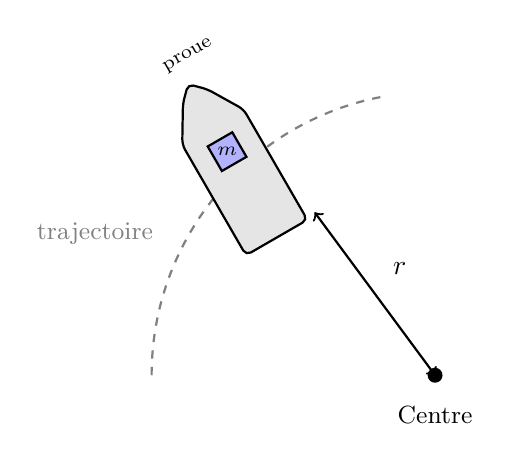
\begin{tikzpicture}[scale=0.9]
    % Vue de dessus - trajectoire courbe
    \draw[dashed, gray, thick] (0, 0) arc (180:100:4);
    \node[gray] at (-0.8, 2) {\small trajectoire};
    
    % Navire (forme de navire vu de dessus, plus grand)
    \begin{scope}[rotate=30, shift={(2.5, 2)}]
        \draw[thick, fill=gray!20, rounded corners=2pt] (-0.5, -1.2) -- (0.5, -1.2) 
            -- (0.5, 0.6) -- (0.2, 1.1) -- (0, 1.3) -- (-0.2, 1.1) -- (-0.5, 0.6) -- cycle;
        % Caisse sur le pont
        \draw[thick, fill=blue!30] (-0.2, 0) rectangle (0.2, 0.4);
        \node[font=\scriptsize] at (0, 0.2) {$m$};
        % Direction proue
        \node[font=\scriptsize, above] at (0, 1.3) {\rotatebox{30}{proue}};
    \end{scope}
    
    % Centre du virage
    \fill (4, 0) circle (3pt);
    \node[below] at (4, -0.3) {\small Centre};
    
    % Rayon
    \draw[thick, <->] (4, 0) -- (2.3, 2.3);
    \node at (3.5, 1.5) {$r$};
\end{tikzpicture}
\end{center}

\textbf{a) Force centripète nécessaire pour le navire}
\[
    F_c = m\frac{v^2}{r} = \SI{5e6}{kg} \times \frac{(10)^2}{500} = \SI{5e6}{kg} \times \SI{0{,}2}{m/s^2} = \boxed{\SI{1e6}{N} = \SI{1}{MN}}
\]

Cette force est fournie principalement par la pression latérale de l'eau sur la coque en dérive (voir l'encadré précédent).

\textbf{b) Glissement de la caisse}

L'accélération centripète subie par la caisse est :
\[
    a_c = \frac{v^2}{r} = \frac{100}{500} = \SI{0{,}2}{m/s^2}
\]

Force centripète nécessaire pour la caisse :
\[
    F_{c,caisse} = m_{caisse} \times a_c = 200 \times 0{,}2 = \SI{40}{N}
\]

Frottement maximal disponible :
\[
    f_{s,max} = \mu_s m_{caisse} g = 0{,}4 \times 200 \times 9{,}81 = \SI{785}{N}
\]

Comme $\SI{40}{N} \ll \SI{785}{N}$, le frottement est largement suffisant. \textbf{La caisse ne glisse pas.}

\textbf{Remarque :} Lors de manœuvres d'urgence (virage serré à haute vitesse), $a_c$ peut devenir beaucoup plus grand, d'où l'importance critique de l'arrimage de la cargaison! Une caisse mal arrimée qui glisse peut causer des dommages ou déstabiliser le navire.
\end{exemple}

% -----------------------------------------------------------------------------
\subsubsection{Câble de grue en rotation}
% -----------------------------------------------------------------------------

\begin{exemple}{Charge suspendue à une grue qui pivote}{grue-pivot}
Une grue de navire pivote pour déplacer une charge de $m = \SI{500}{kg}$. Le câble fait un angle $\theta$ avec la verticale pendant la rotation. Si le rayon de rotation est $r = \SI{8}{m}$ et la période de rotation est $T = \SI{10}{s}$, quel angle fait le câble avec la verticale?

\tcblower

\textbf{\underline{Analyse}}

Pendant la rotation, la charge décrit un cercle horizontal. La tension dans le câble doit :
\begin{itemize}
    \item Compenser le poids (composante verticale)
    \item Fournir la force centripète (composante horizontale)
\end{itemize}

\begin{center}
\begin{tikzpicture}[scale=1.0]
    % Axe de rotation (mât de grue)
    \draw[very thick, gray] (0, 3.5) -- (0, 0);
    \fill[gray] (0, 3.5) circle (3pt);
    \node[gray, above] at (0, 3.6) {\small Mât};
    
    % Verticale de référence
    \draw[dashed, gray] (0, 3.5) -- (0, 0.5);
    
    % Câble (à angle theta ~ 25° par rapport à la verticale)
    \draw[thick, brown] (0, 3.5) -- ({2.5*sin(25)}, {3.5-2.5*cos(25)});
    
    % Angle theta (arc entre la verticale et le câble)
    \draw[thick, ->] (0, 2.5) arc (270:{270+25}:1.0);
    \node at ({0.6*sin(12)}, 2.2) {$\theta$};
    
    % Charge
    \draw[thick, fill=blue!30] ({2.5*sin(25)-0.35}, {3.5-2.5*cos(25)-0.35}) 
        rectangle ({2.5*sin(25)+0.35}, {3.5-2.5*cos(25)+0.05});
    \node at ({2.5*sin(25)}, {3.5-2.5*cos(25)-0.15}) {\small $m$};
    
    % DCL (à droite, bien séparé)
    \begin{scope}[xshift=6cm, yshift=1.5cm]
        \node[font=\bfseries\small, above] at (0, 2.2) {DCL};
        \fill[blue!50] (0, 0) circle (4pt);
        
        % Tension (vers le haut-gauche, le long du câble)
        \draw[-{Stealth[length=3mm]}, very thick, orange] (0, 0) -- ({-2.0*sin(25)}, {2.0*cos(25)});
        \node[orange, above left] at ({-1.0*sin(25)}, {1.0*cos(25)+0.3}) {$\vec{T}$};
        
        % Composante verticale de T
        \draw[dashed, orange, thin] ({-2.0*sin(25)}, {2.0*cos(25)}) -- (0, {2.0*cos(25)});
        \node[orange, font=\scriptsize, right] at (0.1, {2.0*cos(25)-0.15}) {$T\cos\theta$};
        
        % Composante horizontale de T
        \draw[dashed, orange, thin] ({-2.0*sin(25)}, {2.0*cos(25)}) -- ({-2.0*sin(25)}, 0);
        \node[orange, font=\scriptsize, left] at ({-2.0*sin(25)-0.1}, 0.5) {$T\sin\theta$};
        
        % Poids (vers le bas)
        \draw[-{Stealth[length=3mm]}, very thick, red] (0, 0) -- (0, -1.5);
        \node[red, left] at (-0.15, -0.8) {$m\vec{g}$};
        
        % Axes (bien séparés à droite)
        \draw[-{Stealth}, thick] (2.0, 0) -- (2.0, 1.5) node[right] {$y$};
        \draw[-{Stealth}, thick] (2.0, 0) -- (0.8, 0) node[below right] {$x$};
        \node[font=\scriptsize, below] at (1.4, -0.15) {(vers centre)};
    \end{scope}
    
    % Trajectoire circulaire (vue de dessus, schématique)
    \draw[dashed, gray] (0, {3.5-2.5*cos(25)-0.15}) ellipse (1.6cm and 0.3cm);
    \node[gray, font=\scriptsize, below] at (0, {3.5-2.5*cos(25)-0.55}) {trajectoire circulaire};
\end{tikzpicture}
\end{center}

\textbf{\underline{Calculs préliminaires}}

Vitesse angulaire :
\[
    \omega = \frac{2\pi}{T} = \frac{2\pi}{10} = \SI{0{,}628}{rad/s}
\]

\textbf{\underline{Équations}}

Selon $y$ (vertical) : $\sum F_y = 0$
\[
    T\cos\theta - mg = 0 \quad \Rightarrow \quad T\cos\theta = mg
\]

Selon $x$ (vers le centre, horizontal) : $\sum F_x = ma_c$
\[
    T\sin\theta = m\omega^2 r
\]

\textbf{\underline{Résolution}}

Divisons :
\[
    \frac{T\sin\theta}{T\cos\theta} = \frac{m\omega^2 r}{mg}
\]
\[
    \tan\theta = \frac{\omega^2 r}{g} = \frac{(0{,}628)^2 \times 8}{9{,}81} = \frac{3{,}15}{9{,}81} = 0{,}321
\]
\[
    \theta = \arctan(0{,}321) = \boxed{17{,}8\si{\degree}}
\]

\textbf{Tension dans le câble :}
\[
    T = \frac{mg}{\cos\theta} = \frac{500 \times 9{,}81}{\cos 17{,}8\si{\degree}} = \frac{4905}{0{,}952} = \boxed{\SI{5150}{N}}
\]

La tension est légèrement supérieure au poids ($\SI{4905}{N}$) à cause de la composante centripète.
\end{exemple}

\begin{pratiqueautonome}[title=Passager sur le pont d'un traversier]
Un traversier effectue un virage de rayon $r = \SI{300}{m}$ à une vitesse de $v = \SI{8}{m/s}$ (environ 16 nœuds). Un passager de $\SI{70}{kg}$ se tient debout sur le pont.

\begin{enumerate}
    \item Quelle est l'accélération centripète subie par le passager?
    \item Quelle force horizontale le pont doit-il exercer sur les pieds du passager?
    \item Si le coefficient de frottement statique entre ses chaussures et le pont est $\mu_s = 0{,}6$, risque-t-il de glisser?
    \item À quelle vitesse le passager commencerait-il à glisser?
\end{enumerate}

\espaceresolution[5cm]

\tcblower
\textbf{Réponses :}
\begin{enumerate}
    \item $a_c = \dfrac{v^2}{r} = \dfrac{64}{300} = \SI{0{,}213}{m/s^2}$
    \item $F_c = ma_c = 70 \times 0{,}213 = \SI{14{,}9}{N}$ (frottement statique)
    \item $f_{s,max} = \mu_s mg = 0{,}6 \times 70 \times 9{,}81 = \SI{412}{N}$. Comme $\SI{14{,}9}{N} \ll \SI{412}{N}$, \textbf{non}, il ne glisse pas.
    \item $v_{max} = \sqrt{\mu_s g r} = \sqrt{0{,}6 \times 9{,}81 \times 300} = \SI{42}{m/s} \approx 82$ nœuds (impossible pour un traversier!)
\end{enumerate}
\end{pratiqueautonome}

% =============================================================================
\subsection{Résumé : mouvement circulaire}
\label{subsec:resume-circulaire}
% =============================================================================

\begin{center}
\begin{tikzpicture}
    % Boîte principale
    \node[draw=bleuimq, fill=bleuclair, rounded corners=5pt, text width=14cm, align=left, inner sep=10pt] {
        \textbf{\large Points clés du mouvement circulaire} \\[0.5em]
        
        \textbf{1. L'accélération centripète existe toujours} en mouvement circulaire : $a_c = \dfrac{v^2}{r}$ \\[0.5em]
        
        \textbf{2. La force centripète} est la force \textit{résultante} vers le centre : $F_c = ma_c = m\dfrac{v^2}{r}$ \\[0.5em]
        
        \textbf{3. Ce n'est PAS une nouvelle force!} C'est le nom donné à la composante centripète des forces réelles (tension, frottement, normale, gravité...) \\[0.5em]
        
        \textbf{4. La « force centrifuge » n'existe pas} dans un référentiel inertiel. C'est l'effet de l'inertie. \\[0.5em]
        
        \textbf{5. Méthode :} Choisir un axe vers le centre, puis $\sum F_{\to centre} = m\dfrac{v^2}{r}$
    };
\end{tikzpicture}
\end{center}